\documentclass{article}
\usepackage[utf8]{inputenc}
\usepackage[spanish]{babel}
\usepackage{subcaption}
\usepackage{graphicx}
\usepackage{pgffor}
\graphicspath{ {images/} }

\usepackage{listings}
\lstdefinestyle{code}{
language=Octave,
frame=single,
breakatwhitespace=true,
breaklines=true,
basicstyle=\small\ttfamily,
tabsize=4,
numbers=left,
numberstyle=\tiny,
columns=fullflexible
}
\lstdefinestyle{snippet}{
language=Octave,
breakatwhitespace=true,
breaklines=true,
basicstyle=\small\ttfamily,
}

\addtolength{\textwidth}{1cm}
\addtolength{\textheight}{0.75cm}

\title{Práctica 1}
\author{Héctor Laria Mantecón y Samuel Lapuente Jiménez}
\date{5 de noviembre de 2015}

\begin{document}

\maketitle

\section{Introducción}
El objetivo de esta práctica consiste en el estudio mediante regresión logística para determinar una función con salida entera que decida según unos datos de entrada una salida.

\subsection{Visualización de los datos}
\begin{figure}[h]
\centering
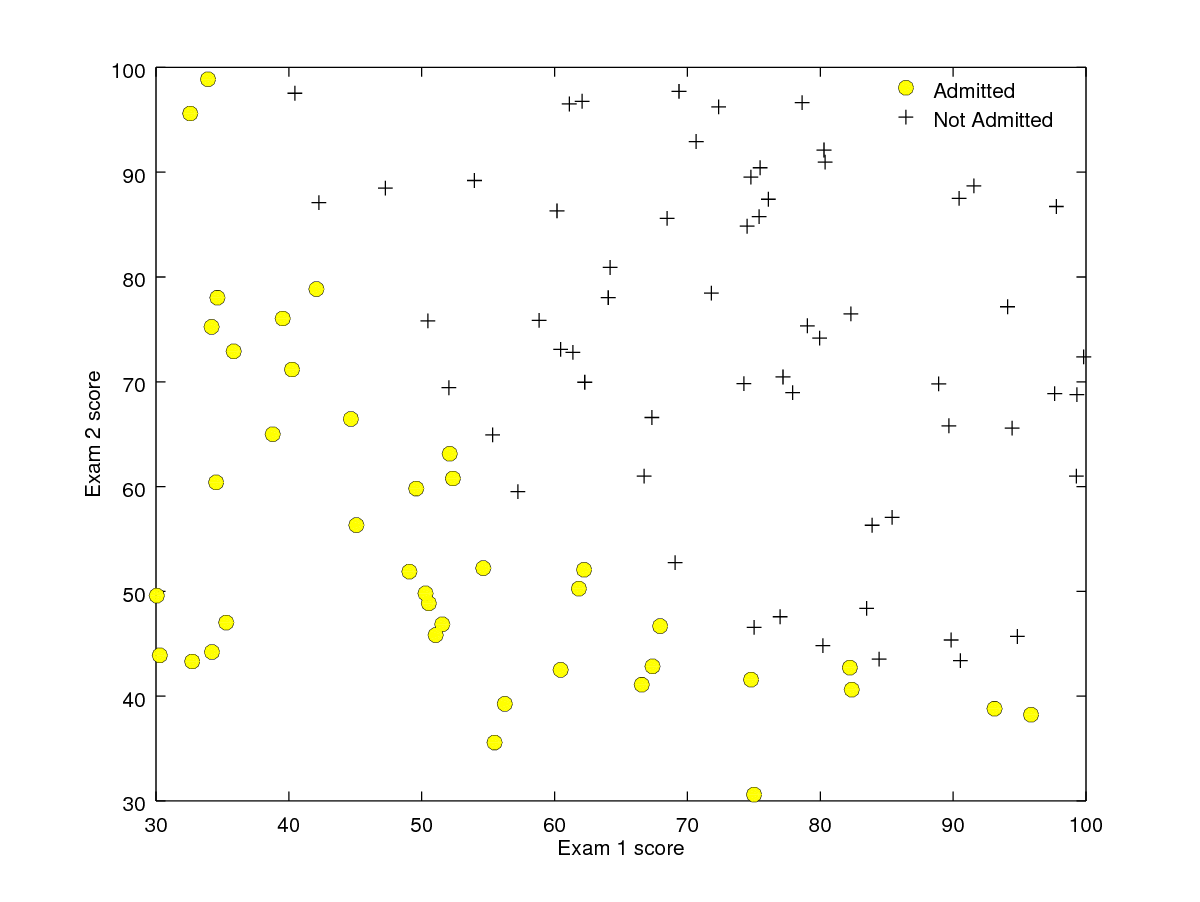
\includegraphics[width=\textwidth]{examples1}
\label{fig:estudio}
\end{figure}

\subsection{Función sigmoide}
Método que calcula la función sigmoide.
\lstinputlisting[style=code]{src/sig.m}

\subsection{Función de coste y gradiente}
\lstinputlisting[style=code]{src/cost.m}

\subsection{Cálculo del valor óptimo}
\lstinputlisting[style=code]{src/uno.m}

\begin{figure}[h]
\centering
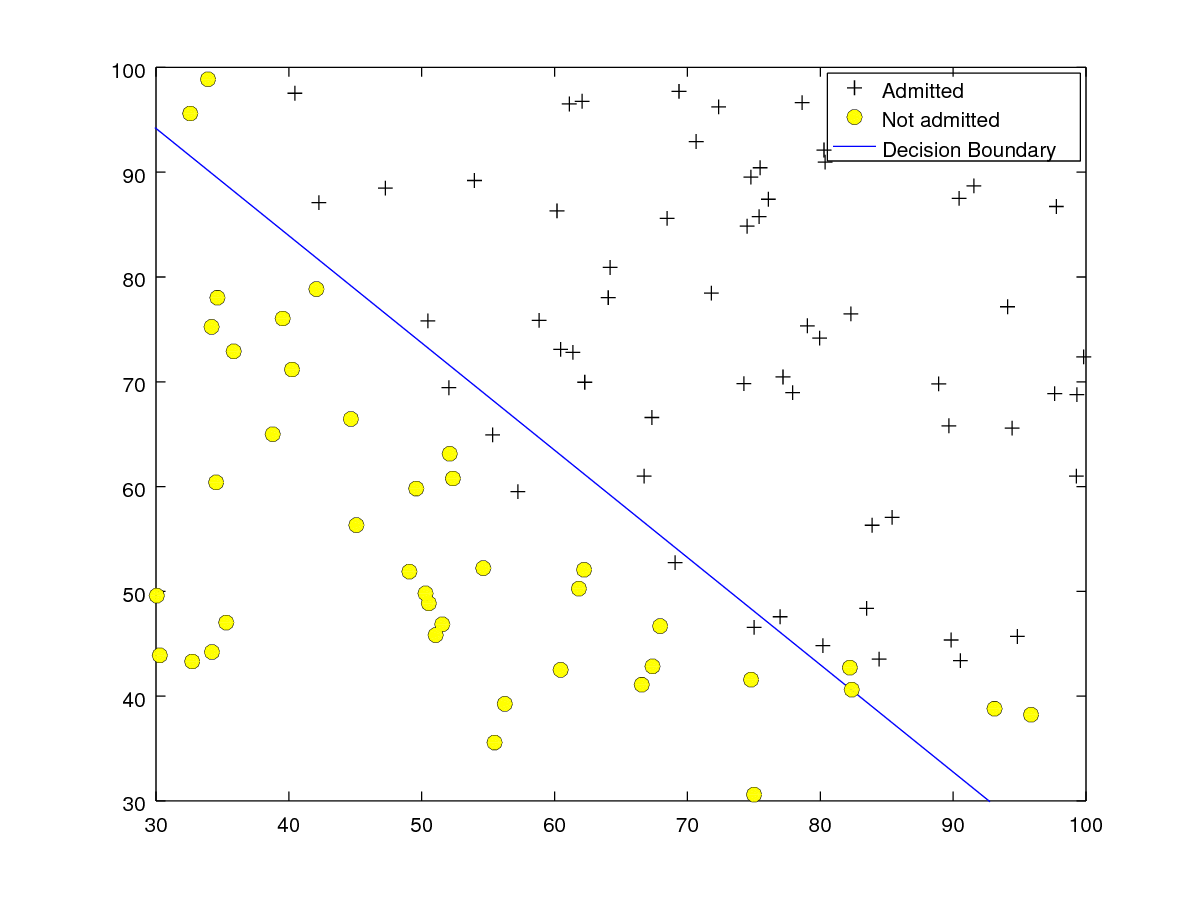
\includegraphics[width=\textwidth]{regresion1}
\label{fig:estudio}
\end{figure}

\subsection{Evaluación de la regresión logística}
Con este método calculamos el porcentaje de aciertos produce el modelo.
\lstinputlisting[style=code]{src/percentage.m}
En nuestro caso, la llamada a esta función en el método {\tt uno.m} devuelve:
\begin{lstlisting}[style=snippet]
Percentage of well classified examples: 89
\end{lstlisting}

\pagebreak
\section{Regresión logística regularizada}
Visualización de los atributos no linealmente separables:
\begin{figure}[h]
\centering
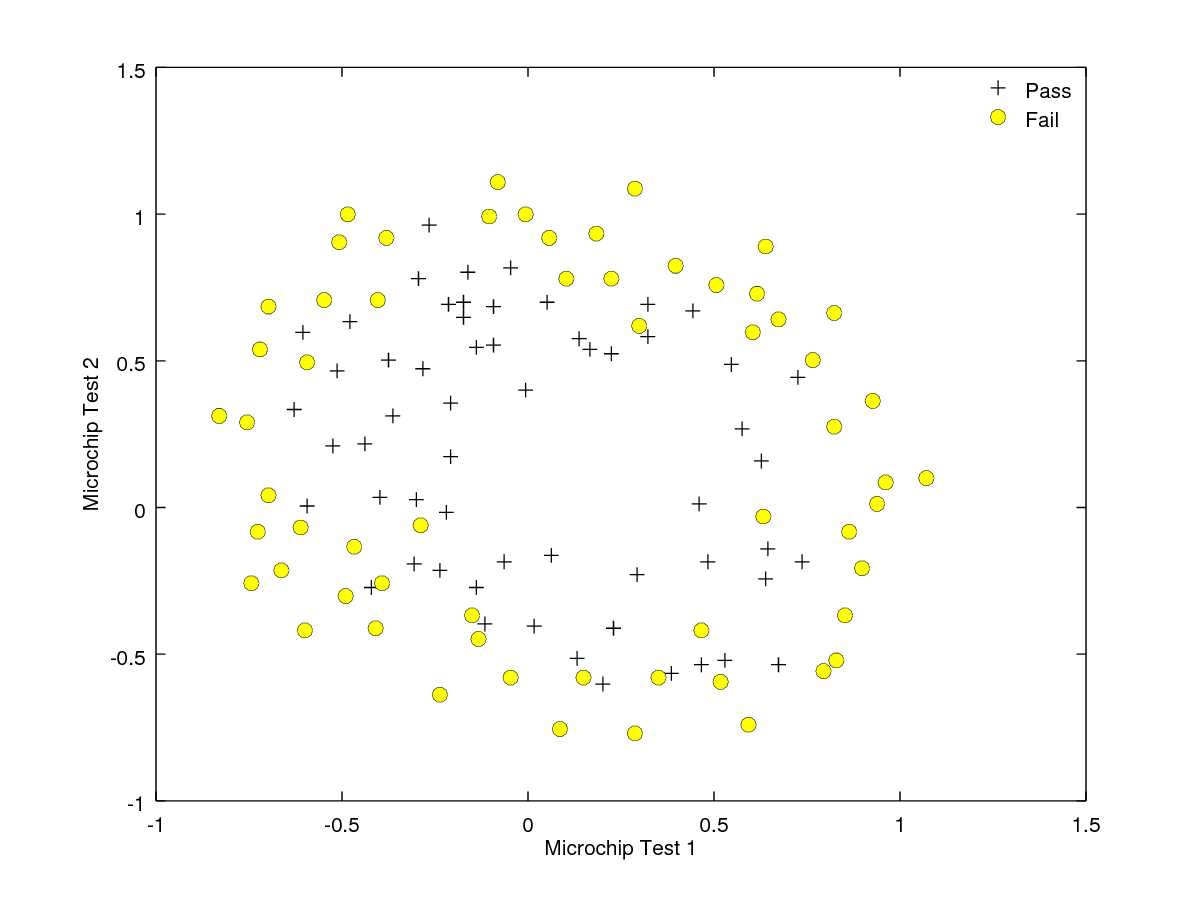
\includegraphics[width=\textwidth]{examples2}
\label{fig:estudio}
\end{figure}

\subsection{Función coste y gradiente}
\lstinputlisting[style=code]{src/costRegulariz.m}

\subsection{Cálculo del valor óptimo}
Usamos este código para calcular los valores $\theta$ óptimos. Usamos {\tt mapFeature(x)} para obtener más atributos. La salida del script es la dada más abajo.
\lstinputlisting[style=code]{src/dos.m}

\begin{figure}[h]
\centering
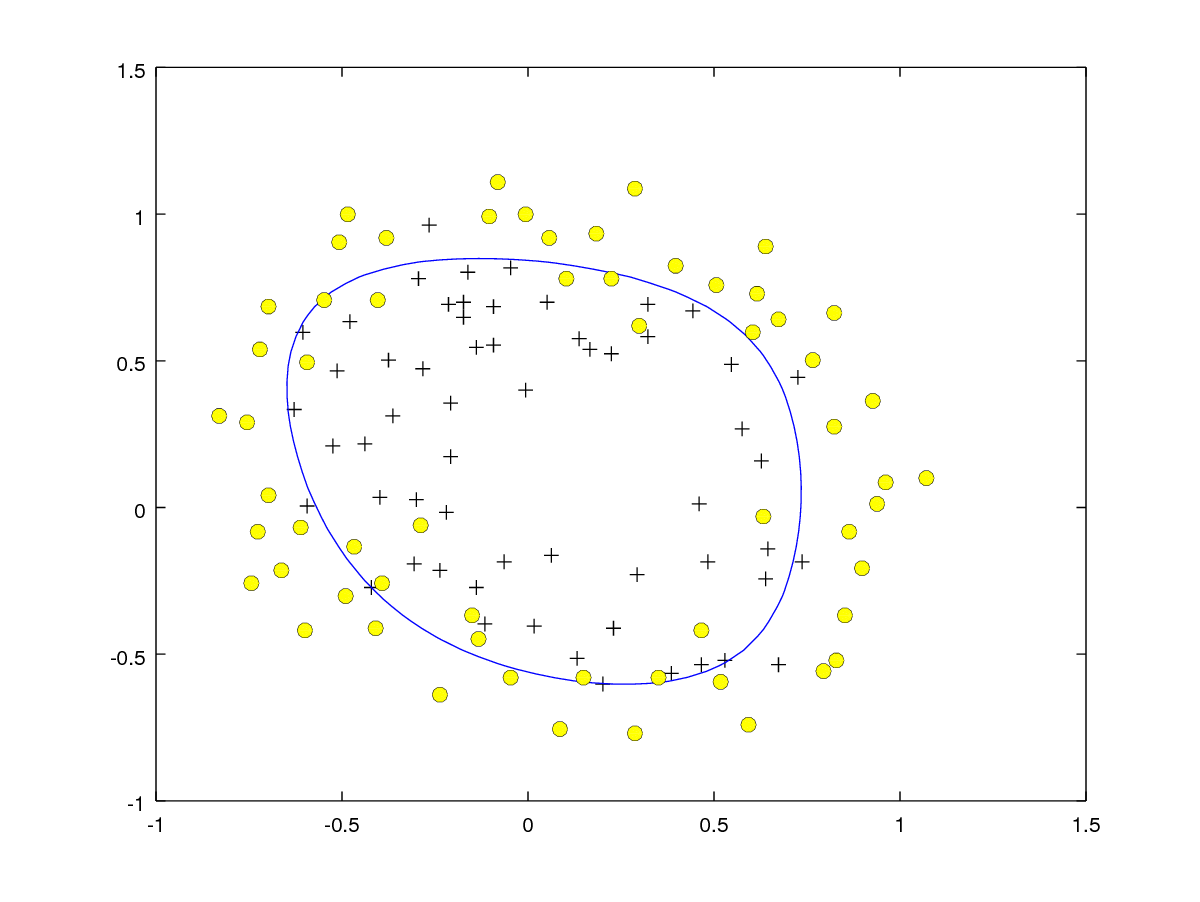
\includegraphics[width=0.55\textwidth]{regresion2}
\label{fig:estudio}
\end{figure}

\begin{lstlisting}[style=snippet]
Percentage of well classified examples: 82.203
\end{lstlisting}

\subsection{Efectos de la regularización}
Ahora experimentamos con los valores de $\lambda$. Para cada gráfica se muestra su valor y el porcentaje de aciertos.

\begin{figure}[h]
\centering
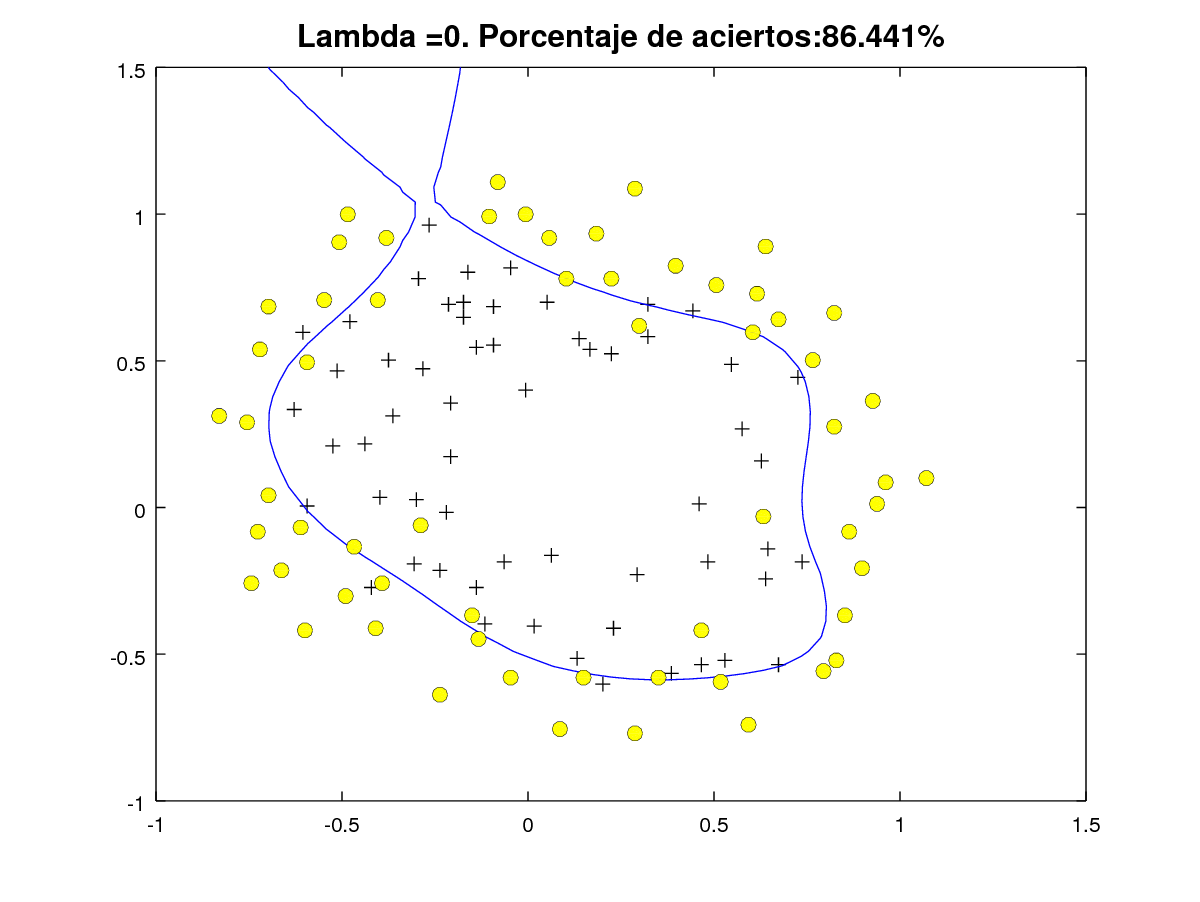
\includegraphics[width=0.7\textwidth]{estudio0}
\label{fig:estudio}
\end{figure}

\begin{figure}[h]
\centering
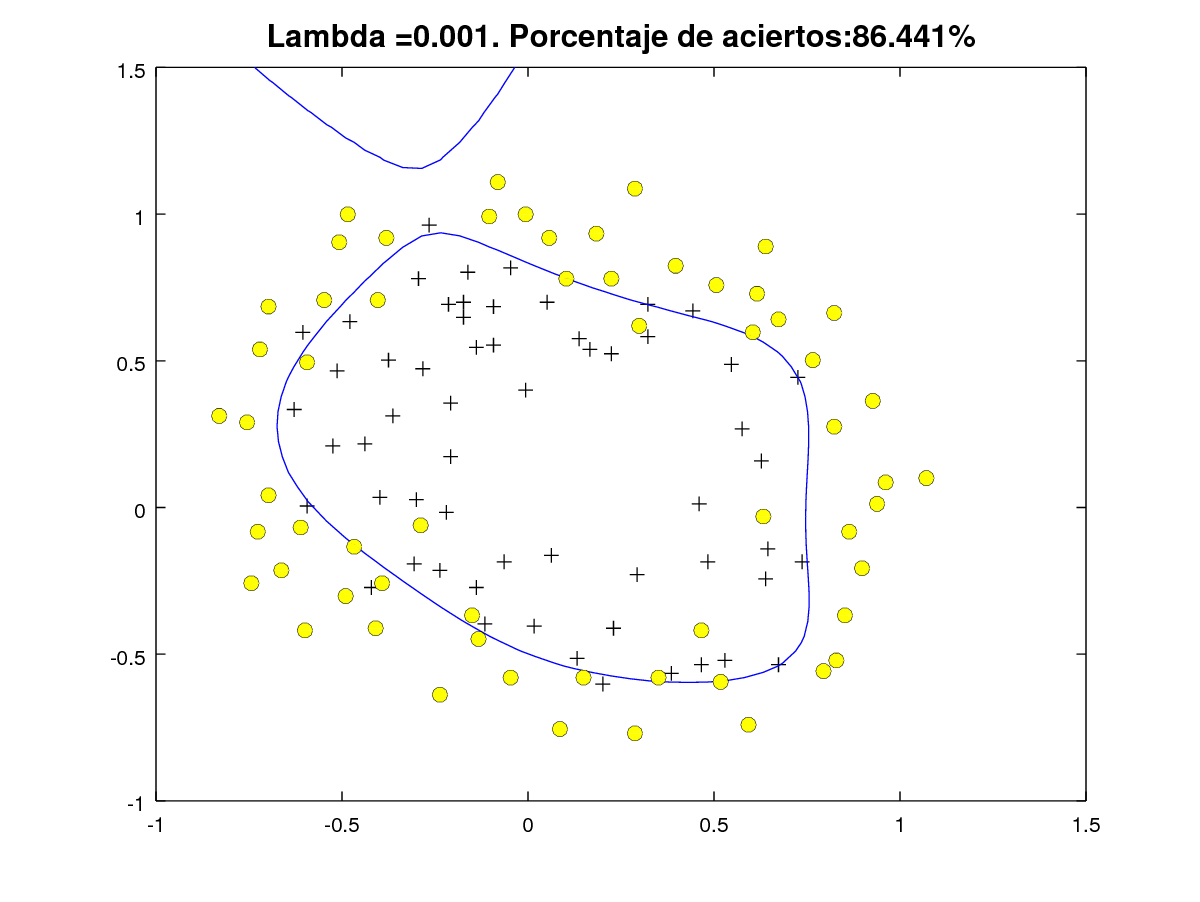
\includegraphics[width=0.7\textwidth]{estudio1}
\label{fig:estudio}
\end{figure}

\begin{figure}[h]
\centering
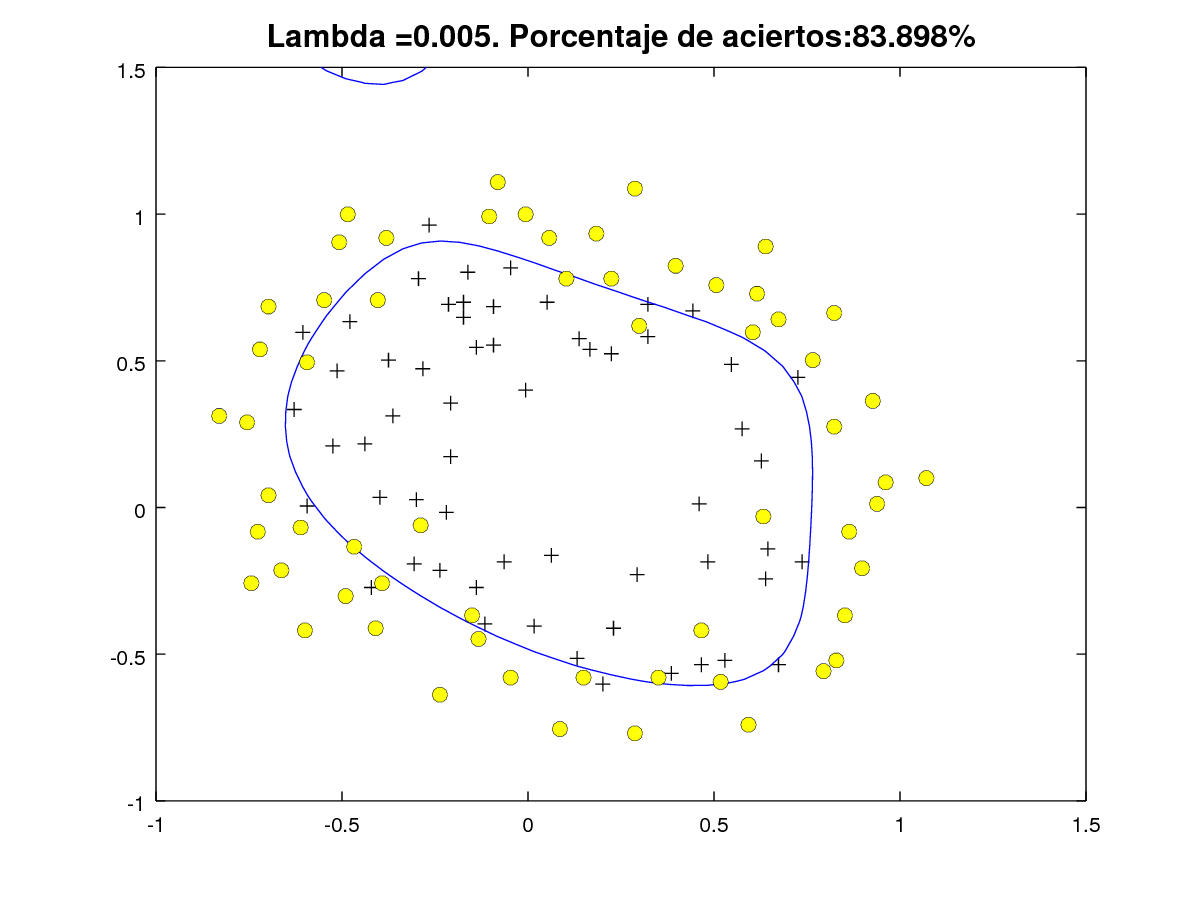
\includegraphics[width=0.7\textwidth]{estudio2}
\label{fig:estudio}
\end{figure}

\begin{figure}[h]
\centering
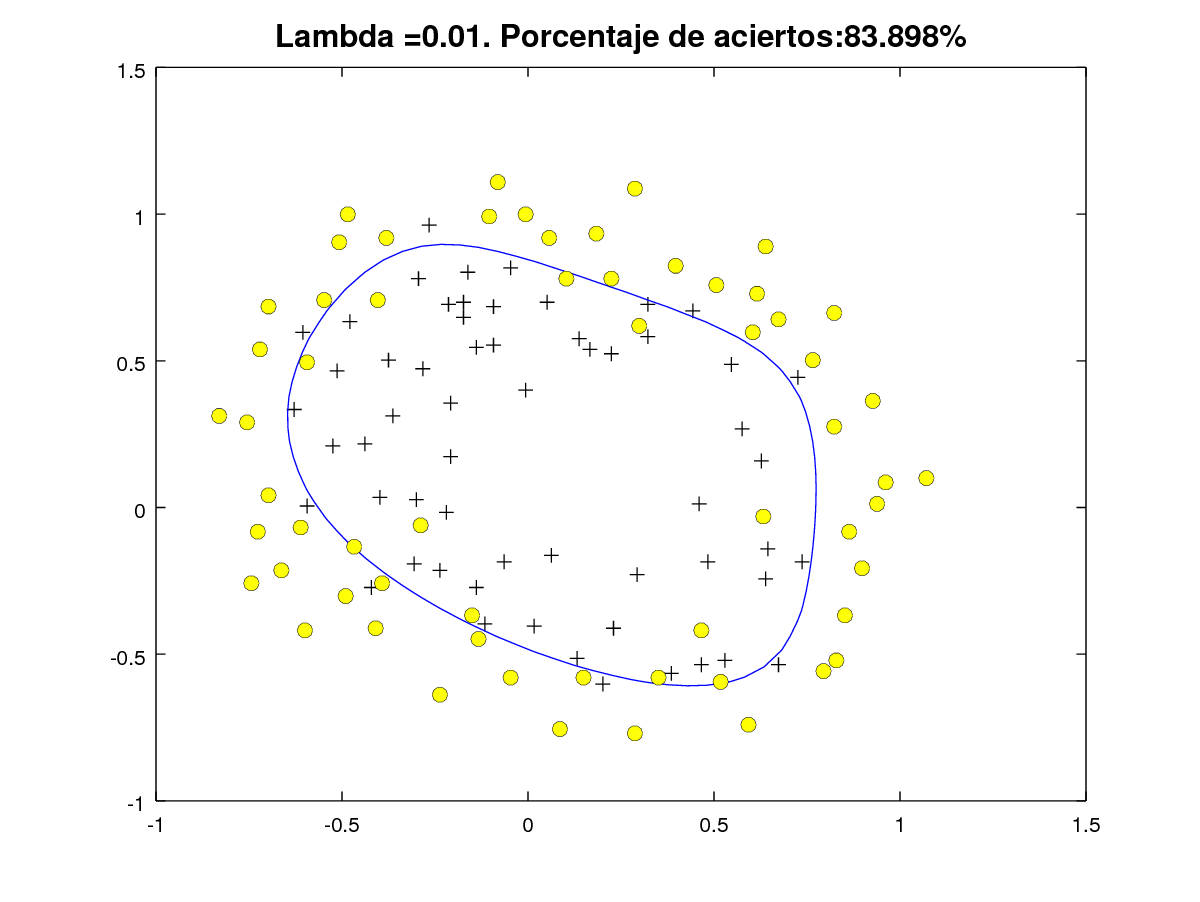
\includegraphics[width=0.7\textwidth]{estudio3}
\label{fig:estudio}
\end{figure}

\begin{figure}[h]
\centering
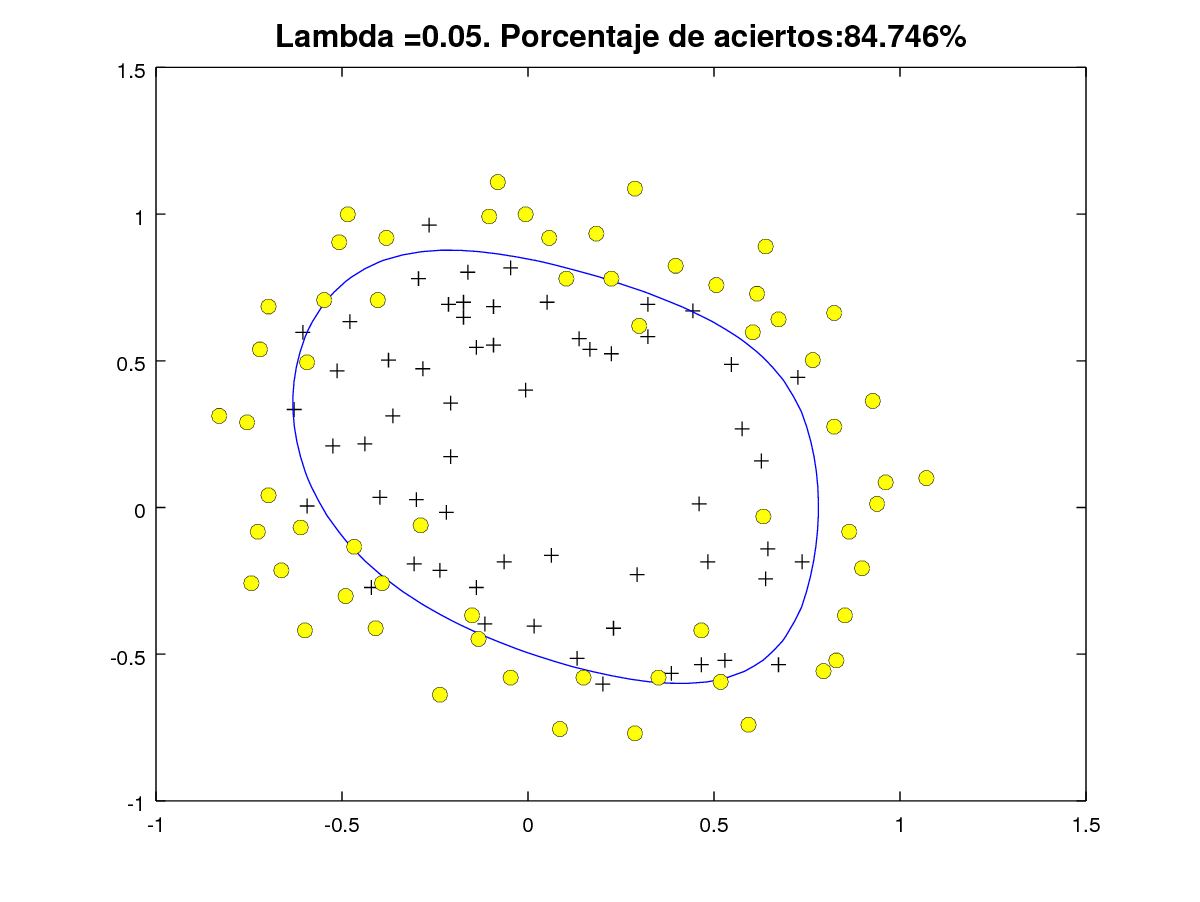
\includegraphics[width=0.7\textwidth]{estudio4}
\label{fig:estudio}
\end{figure}

\begin{figure}[h]
\centering
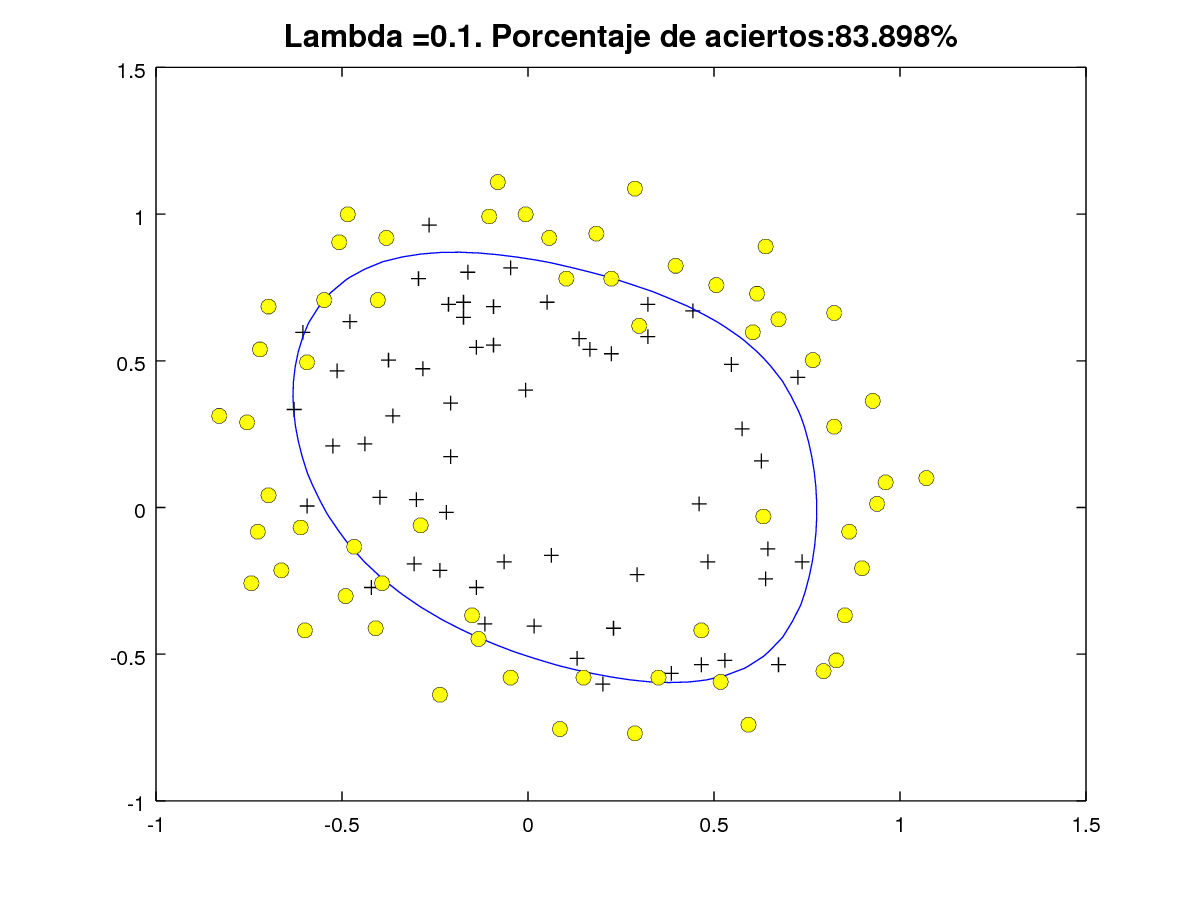
\includegraphics[width=0.7\textwidth]{estudio5}
\label{fig:estudio}
\end{figure}

\begin{figure}[h]
\centering
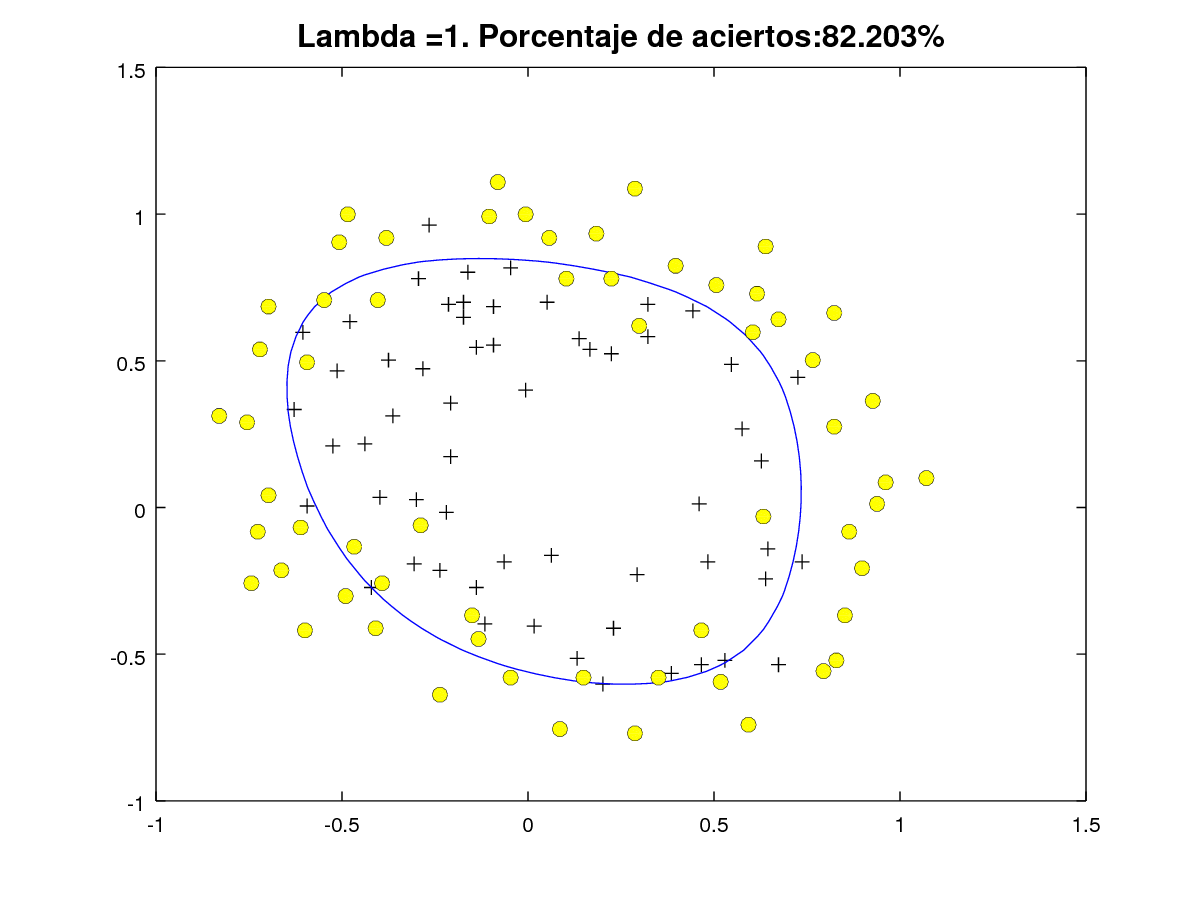
\includegraphics[width=0.7\textwidth]{estudio6}
\label{fig:estudio}
\end{figure}

\begin{figure}[h]
\centering
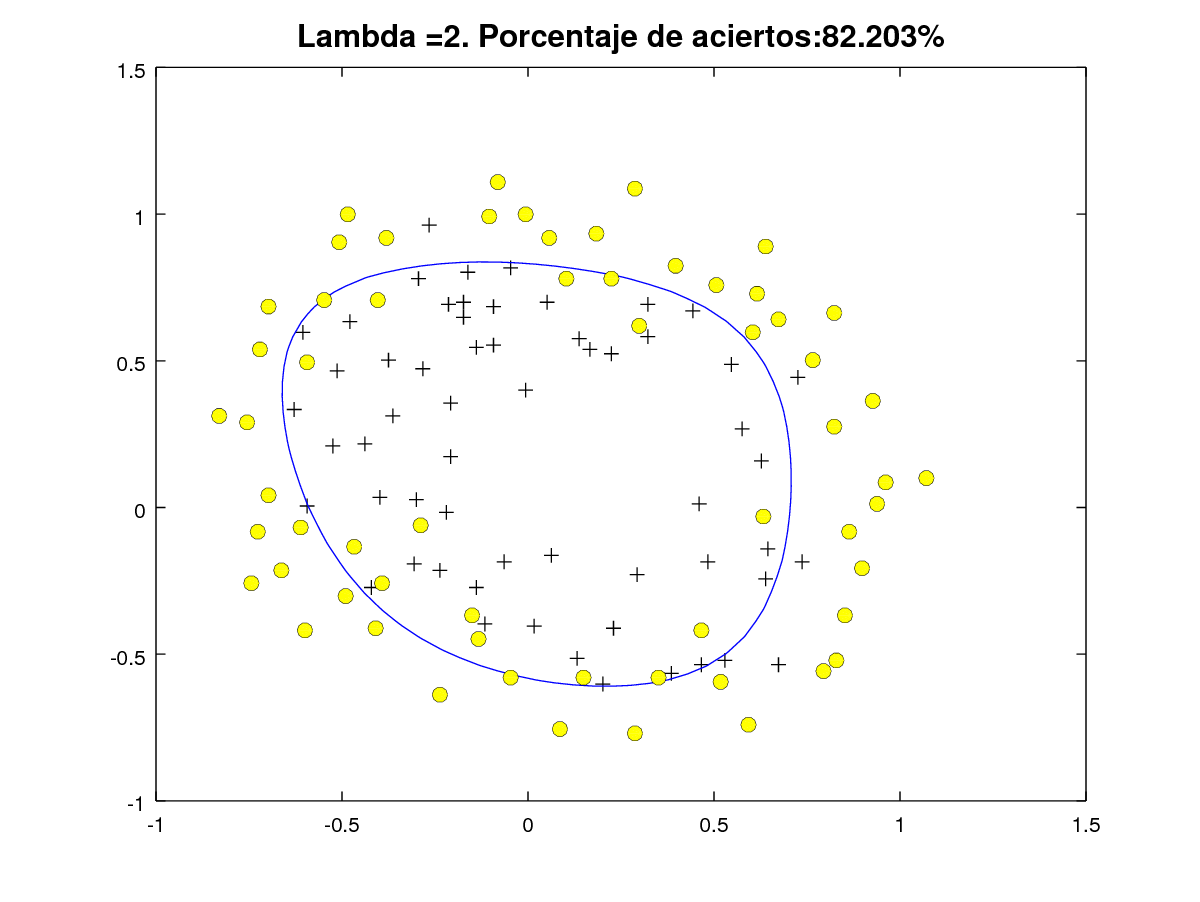
\includegraphics[width=0.7\textwidth]{estudio7}
\label{fig:estudio}
\end{figure}

\end{document}
